\documentclass{article}

% Load packages
\usepackage[a4paper, top=2.5cm, bottom=2.5cm, left=2.5cm, right=2.5cm]{geometry} % set margins
\usepackage[utf8]{inputenc} % unicode support
\usepackage{amsmath,amsfonts,amssymb,amsthm} % maths
\usepackage{mathtools} % maths operators
\usepackage{faktor} % quotient rings
\usepackage{graphicx} % graphics
\usepackage{float} % define floating objects like tables or figures
\usepackage{url} % url
\usepackage{csquotes} % quotes
\usepackage{booktabs} % table lines
\usepackage{enumitem} % spacing of lists
\usepackage[nottoc]{tocbibind} % add bibliography to toc
\usepackage[backend=biber,sorting=none,style=numeric,block=ragged]{biblatex} % references, alternative: style=alphabetic
\usepackage[linesnumbered, ruled]{algorithm2e} % algorithm package
\usepackage{aliascnt} % alias counter package
\usepackage[linktocpage=true, bookmarks=true, bookmarksnumbered=true, pdfpagemode=UseNone, pdfstartview={XYZ null null 1}, colorlinks=false,hidelinks]{hyperref}
\usepackage[noabbrev,capitalize,nameinlink]{cleveref}
\usepackage{todonotes}
\usepackage{lipsum}
\usepackage{subfiles} % multiple subfiles

% spacing
\setlength{\parskip}{1em}
\setlength{\parindent}{0em}
\setlist{nosep}

% variables macro
\newcommand{\etal}{\textit{et. al.}}

% maths operators
\DeclareMathOperator{\ord}{ord}
\DeclarePairedDelimiter{\abs}{\lvert}{\rvert}
\DeclarePairedDelimiter{\norm}{\lVert}{\rVert}
\DeclarePairedDelimiter{\set}{\{}{\}}
\DeclarePairedDelimiter{\angle}{\langle}{\rangle}

% counters
\newaliascnt{mycounter}{algocf} % let "counter" be an alias for "algocf"
\newcommand\addtag{\refstepcounter{mycounter} \tag{\themycounter}}
\numberwithin{equation}{mycounter} % subbordinated equations to mycounter
\numberwithin{table}{mycounter}

% algorithms
\SetKwInput{Initialization}{Initialization}

% theorems environments
\theoremstyle{plain}
\newtheorem{theorem}[mycounter]{Theorem}
\newtheorem{proposition}[mycounter]{Proposition}
\newtheorem{lemma}[mycounter]{Lemma}
\newtheorem{corollary}[mycounter]{Corollary}

\theoremstyle{definition}
\newtheorem{definition}[mycounter]{Definition}
\newtheorem{example}[mycounter]{Example}

\theoremstyle{remark}
\newtheorem*{remark}{Remark}
\newtheorem*{prf}{Proof}

\newtheoremstyle{style1}
    {\topsep} % Space above
    {\topsep} % Space below
    {} % Theorem body font % (default is "\upshape")
    {} % Indent amount
    {\bfseries} % Theorem head font % (default is \mdseries)
    {.} % Punctuation after theorem head % default: no punctuation
    {\newline} % Space after theorem head
    {} % Theorem head spec
\theoremstyle{style1}
\newtheorem{construction}[mycounter]{Construction}
\newtheorem{problem}[mycounter]{Hard Problem}

% cref
\creflabelformat{equation}{#2#1#3} % no parenthesis for equation environment

% url
\def\UrlBreaks{\do/\do-}

% bibliography
\addbibresource{references.bib}

% chapter author
\makeatletter
\newcommand{\chapterauthor}[1]
{
    {\parindent0pt\vspace*{-20pt}
    \linespread{1.1}\large\scshape#1
    \par\nobreak\vspace*{1pt}}
    \@afterheading
}
\makeatother

\title{Article Template}
\author{Sim Jun Jie}

\begin{document}

\maketitle

\begin{abstract}
This is an abstract.
\end{abstract}

\section{Paper Format}
\begin{enumerate}
    \item Background
    \item Notation
    \item Methods
    \item Results
    \item Discussion
    \item Conclusion
\end{enumerate}

\section{Math Environments}

\[ \text{This is an equation.} \addtag \label{eq1} \]

\begin{definition}
    This is a definition. \label{def1}
\end{definition}

\begin{proposition}
    This is a proposition. \label{prop1}
\end{proposition}

\begin{lemma}
    This is a lemma. \label{lemma1}
\end{lemma}

\begin{theorem}
    This is a theorem. \label{theorem1}
\end{theorem}

\begin{algorithm}[H]
    \caption{This is an algorithm.}
    \label{algo1}
    \KwIn {Some inputs}
    \KwOut {Some outputs}
    \Initialization {Some variables}

    \While {condition not met}
    {
        Some code\;
        Some more code\; \label{line1}
    }
    \For {$i = 0$ \KwTo $k$}
    {
        \uIf {some condition holds}
        {
            Do some magic\;
        }
        \Else
        {
            \Return $m$\;
        }
    }
\end{algorithm}

\[ \text{This is an equation.} \addtag \label{eq3} \]

\begin{example}
    This is an example. \label{eg1}
\end{example}

\begin{table}[H]
    \centering
    \begin{tabular}{lcccc}
        \toprule
         & col $1$ & col $2$ & col $3$ & col  $4$ \\
        \midrule
        row $1$ & $(1,1)$ & $(1,2)$ & $(1,3)$ & $(1,4)$ \\
        row $2$ & $(2,1)$ & $(2,2)$ & $(2,3)$ & $(2,4)$ \\
        row $3$ & $(3,1)$ & $(3,2)$ & $(3,3)$ & $(3,4)$ \\
        \bottomrule
    \end{tabular}
    \caption{This is a table.}
    \label{table1}
\end{table}

\begin{example}
    \label{eg2}
    This is a second example.
    \[ \text{With a second equation.} \addtag \label{eq2} \]
\end{example}

\section{Subfiles}
\subfile{sections/subfile}

\section{Citations}
You can cite stuff like \cite{article} and \cite{misc}.
Combined citations look like this \cite{book,incollection}.

Use cref for math environments.
\begin{itemize}
    \item An equation I want to cref \cref{eq1}.
    \item A definition I want to cref \cref{def1}.
    \item A proposition I want to cref \cref{prop1}.
    \item A lemma I want to cref \cref{lemma1}.
    \item A theorem I want to cref \cref{theorem1}.
    \item An algorithm I want to cref \cref{algo1}.
    \item An example I want to cref \cref{eg1}.
    \item A line of code I want to cref \cref{algo1} \cref{line1}.
\end{itemize}

Note that autoref does not work properly.
There is a autoref warning \enquote{No autoref name for \enquote{mycounter}} occurs.
The recommended fix would be to rename counters.
See \url{http://tex.stackexchange.com/questions/256672/autoref-does-not-seem-to-be-working-properly} for details.
However, using cref seems to be simpler.

\section{Images}
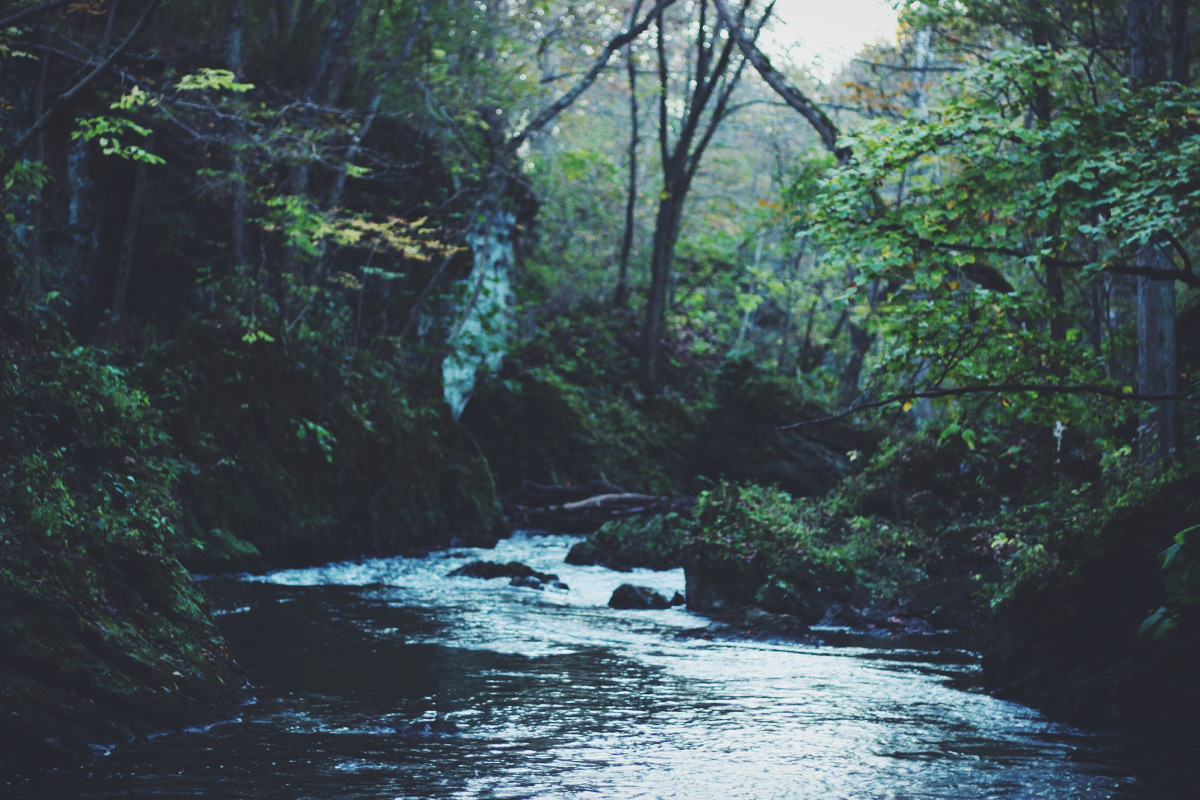
\includegraphics[width=1\textwidth]{stream.jpg}

\nocite{*}
\printbibliography[title={Reference}]

\end{document}